\documentclass[a4paper]{article}

\usepackage[english]{babel}
\usepackage[utf8]{inputenc}
\usepackage{amsmath}
\usepackage{graphicx}
\usepackage[colorinlistoftodos]{todonotes}
\usepackage{hyperref}
\setlength{\parskip}{1em}
\setlength{\parindent}{0em}
\graphicspath{ {./images/} }

\title{Simultaneous Localization and Mapping}

\author{Shabnam Sahay}

\date{June 2020}

\begin{document}
\maketitle

These notes are a summary of my learning from the SLAM course videos offered by Cyrill Stachniss. Through these, I aim to provide an overview of robot mapping, SLAM, and ultimately its practical implementation via the Extended Kalman filter algorithm.

%%%%%%%%%%%%%%%%%%%%%%%%%%%%%%%%%%%%%%%%%%%%

\section{Introduction to Robot Mapping}

\subsection{Important Terms}

Robot: a device which moves through the environment. It has some mechanical means that allows it to move. It is also equipped with sensors. The controls and sensor inputs are exploited to gain knowledge about the environment.

Mapping: modeling the environment. A map is some form of representation of the environment, able to be used for decision-making.

State estimation: knowing the position of the robot of the environment, the positions of some nearby landmarks, and using this to estimate the current state of the robot in the environment e.g. its position, the position of landmarks, etc. One way to do estimation is via a recursive base filter.

Localization: estimation of the location of the robot in relation to the world - the x,y,z coordinates, as well as the angular orientation. The location is sometimes also called the pose.

Mapping: having sensor data, and using it to estimate a model of the environment, i.e. to map it. To be able to map, we must know the position of the sensor itself.

SLAM: when the position of the sensor itself is not certain, SLAM is required. It simultaneously estimates the position of the robot itself, as well as the positions of nearby landmarks in the environment.

Navigation: the ability of the robot to make decisions related to which path to choose to go from one location to another. Usually limited to xyz movement.

Motion planning: connected to navigation. It entails seeking the optimal path to move from one location to another. It may not always involve rigid xyz movement, and allows one to plan a trajectory or a system of states that need to be moved through in order to change locations.

\subsection{What is SLAM?}

SLAM involves computing different positions of the robot at different points in time, as well as computing and updating a map or model of the environment simultaneously.

\begin{itemize}
    \item Localization: estimating the robot's location or trajectory. 
    \item Mapping: building a map
    \item SLAM: mapping and localizing simultaneously
\end{itemize}

In practical applications, one almost always needs to use SLAM - localization or mapping on their own are not accurate enough. Even if the ultimate goal is just something relatively simple, such as modelling the environment, SLAM is needed to do the job effectively.

\textbf{Localization example}

A landmark is something the robot can observe and recognise. As seen, localization involves knowing all the landmarks' positions at a point in time, and using them to find out where the robot itself is.

Let us look at a brief example of how localization works. Suppose due to some mismatches in the wheel dimensions, the robot thinks it is turning left, but it actually ends up turning right. After some movement in the new direction, it checks its distance from a previously known landmark, and realises that there is a difference between what it thinks the distance should be, and what it actually is. It uses this realisation to make a correction in its pose, and attempts to bring the estimated and actual poses closer to each other. The amount of correction depends on the accuracy of its sensors and the accuracy of its motion execution. How much weight we give to each of these depends on which one gives more precise data.

\textbf{Mapping example}

In this case, the motion execution is perfect, so the exact location of the robot itself is known. The sensors are used to continually detect the positions of the landmarks. Sensor data is often noisy, and in the ideal case the degree of accuracy of the sensors is known - for example, the actual landmark has a 95\% chance of being within 10 cm of the detected position. This data can then be used to drawn an uncertainty ellipse around the detected position, and thus model the environement.

\textbf{SLAM example}

Looking back to the localization example, in a practical situation, when the robot's actual direction becomes different from the direction it thinks it is moving in, it is usually not able to realise this accurately. This is because the position of the landmark is generally not known to it from before, and hence it is not able to use the difference in the estimated and actual position to correct its trajectory. If we consider ideal trajectory accuracies:

Trajectory accuracy: Localization $>$ Mapping $>$ SLAM

However, for good localization, we need a perfect map or model of the environment. Conversely, for good mapping, we need extremely precise data on the location/pose estimate of the robot. Thus the use of either one becomes a type of chicken-and-egg problem.

This shows the high inter-dependency of localization and mapping on each other: they cannot be decoupled. This is why SLAM, i.e. simultaneous localization and mapping, is used for autonomous navigation.

\textbf{SLAM applications}

\begin{itemize}
    \item At home: hoovers, lawn mowers
    \item Air: surveillance with UAVs; crops, traffic, etc.
    \item Underwater: reef monitoring
    \item Underground: exploration of mines, catacombs, etc.
    \item Space: terrain mapping for localization
\end{itemize}

Note: If the robot moves randomly while mapping the environment, there is a reasonable chance that it will miss some areas. This is because the mapping is a passive process - the SLAM system doesn't tell the robot \emph{where} to go to do its mapping.

\subsection{Defining the SLAM problem}

\textbf{Given}

\begin{itemize}

    \item The robot's controls
    
    $u_{1:T} = {u_1, u_2, u_3,...,u_T}$
    
    These are control commands. For example, $u_T$ may be a command to move one metre forward. They are closely related to the odometry of the robot, with some important distinctions.
    
    A control command is something that one physically sends to the robot, whereas odometry is based on the feedback that the robot sends back based on its motion (e.g. an encoder on the wheels counting the number of revolutions, telling us that the robot actually moved only 99 cm).
    
    In theory, use of the control commands is enough to direct motion.
    
    \item Observations
    
    $z_{1:T} = {z_1, z_2, z_3,...,z_T}$
    
    These observations are indexed based on the time elapsed. They could be laser scans indicating the proximity to the closest obstacle, camera images detecting landmarks, etc.
    
\end{itemize}

\textbf{Wanted}

\begin{itemize}

    \item Map of the environment
    
    $m$: an accurate model of the environment.
    
    \item Path of the robot
    
    $x_{0:T} = {x_0, x_1, x_2,...,x_T}$
    
    The path variables start from the index 0, because each control command connects two poses. Suppose we have two commands $u_1$ and $u_2$: then the robot will change its pose two times, first from $x_0$ to $x_1$, and then $x_1$ to $x_2$. So $x_0$ in a sense acts as an origin, creating a frame of reference for the location of the robot.
    
\end{itemize}

Both these wanted quantities are highly likely to contain errors when obtained - these errors may be observational, or based on bad data associations, or so on. This is where the use of probabilistic approaches comes in.

\subsection{Probabilistic approaches}

It is wrong to assume that one knows exactly where the robot is. Even if the motion execution system is extremely accurate, there are always errors that creep in - even if they are extremely small, the uncertainty always remains. As the robot moves for longer times and over greater distances, the errors and uncertainty accumulate.

Due to this uncertainty in the robot's motions and observations, probability theory is used to explicitly represent and model the uncertainty.

\textbf{In the probabilistic world}

Estimation of the robot's path and the environment's map involves use of the following probability distribution:

$p(x_{0:T},m|z_{1:T},u_{1:T})$

where
\begin{itemize}
    \item p: probability distribution
    \item $x_{0:T}$: path/trajectory of the robot through its environment; the pose of the robot at discrete points of time
    \item $m$: the environment map
    \item $|$ : given that
    \item $z_{1:T}$: observations
    \item $u_{1:T}$: control commands/odometry observations
\end{itemize}

The ultimate aim is to be able to estimate this probability distribution. The approach we use will change based on the assumptions we make. All estimation techniques make some or the other assumptions. Some may be restrictive, whereas some may be easier to implement or more efficient.

\textbf{Graphical model}

The robot's state is often depicted graphically, as shown.

\begin{center}
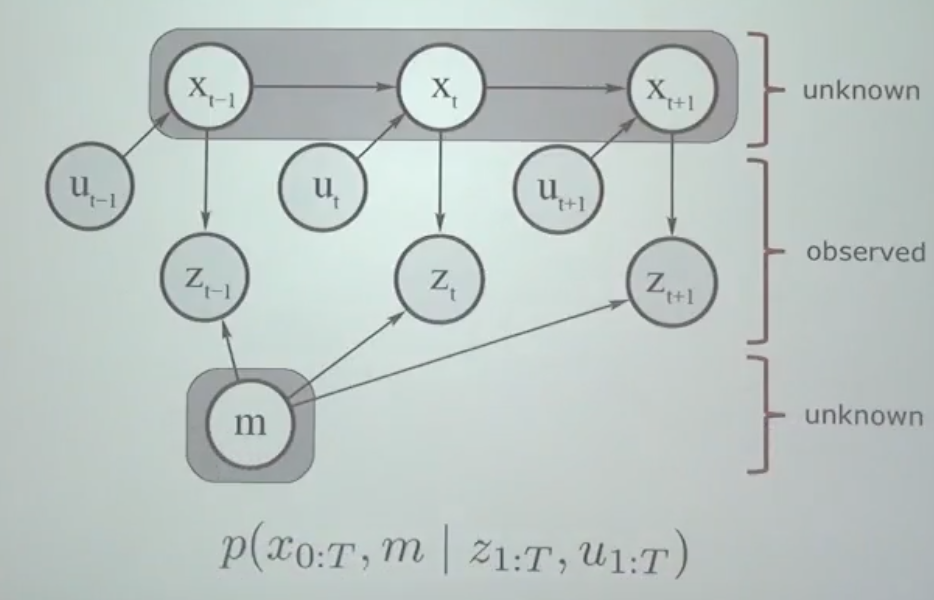
\includegraphics[scale=0.5]{graph-mod}
\end{center}

The arrows represent dependencies; an arrow from $a$ to $b$ indicates that $a$ influences $b$. For example,  we can see that the observations made at a point depend both on the sensor's position, and the landmarks' positions.

This graph represents full SLAM; estimating both the full trajectory of the robot as well as what the environment is. In contrast, online SLAM only estimates the current pose.

\textbf{Full SLAM vs. Online SLAM}

\begin{itemize}

    \item Full SLAM estimates the entire path/trajectory and the map.
    
    $p(x_{0:T}, m | z_{1:T}, u_{1:T})$
    
    \item Online SLAM seeks to recover only the most recent pose.
    
    $p(x_{t}, m | z_{1:t}, u_{1:t})$
    
\end{itemize}

Online SLAM thus estimates only the current pose, and the map built up to the current point, based on all the previously collected sensor data. This is what most robots will use to decide where they are and where they want to go.

Most real-world robot applications will use online SLAM, since it isn't practical to collect all the sensor data throughout the movement and then estimate the poses afterwards - one wants to do it while the robot is moving.

\begin{center}
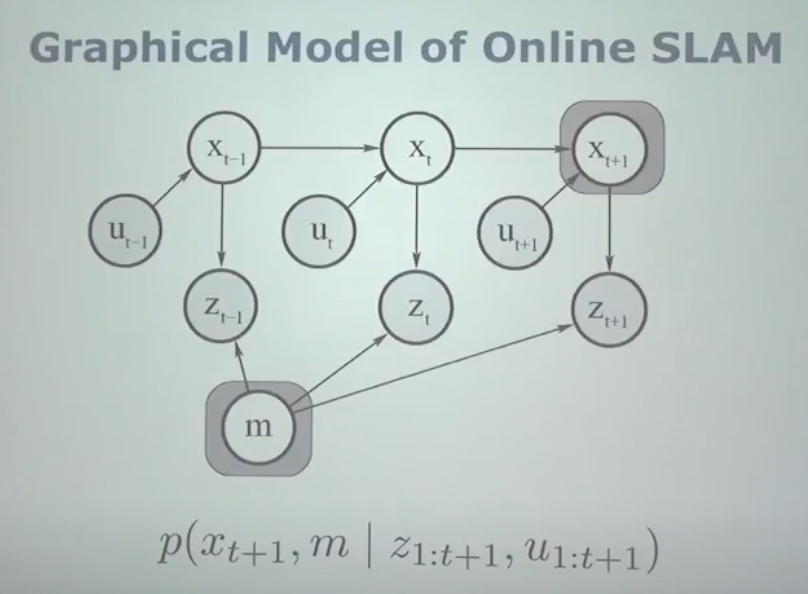
\includegraphics[scale=0.5]{online-slam}
\end{center}

Using online SLAM means marginalizing out the previous poses. The integrals are typically solved recursively, one at a time.

$p(x_{t}, m | z_{1:t}, u_{1:t})$ = 
$$\int_{x_0} \ldots \int_{x_{t-1}} p(x_{0:t}, m | z_{1:t}, u_{1:t}) dx_{t-1} \ldots dx_0 $$

So the map of the environment is the integral of all the possible positions, over $x_0$, over $x_1$, and so on. Integrating out the previous estimations together gives a joint probability distribution for the entire movement up to that point.

Note that representing the probability in the form of such an integral simply makes use of the following property:

$$P(A|B) = \int_{all B} P(A|B) dB$$

\subsection{Why is SLAM a hard problem?}

\begin{itemize}
    \item Robot path and map are both unknown
    \item Map and pose estimates are highly correlated
    \item The mapping between observations and the map itself is unknown
    \item Wrong data associations can have catastrophic consequences (divergence)
\end{itemize}

As seen, motion increases the uncertainty - as the robot moves, one needs to combine the uncertainty created by the robot's pose probabilities with the landmark's position probabilities.

As the robot moves further and re-observes certain landmarks, it can use these observations to make corrections in its estimates and thus improve accuracy.

However, if some landmarks are identical, the robot may confuse two or more landmarks, and cause bad data associations. Uncertainty in the pose estimate also changes the set of landmarks that may be thought of as being observed at that moment.

Hence if one makes a wrong association, a wrong estimate of the uncertainty will be obtained.

\subsection{Taxonomy of the SLAM problem}

\textbf{Kinds of maps estimated}

\begin{itemize}
    \item Volumetric: gives a physical structure of all the surfaces being mapped, or identifies which space is free and which is occupied by obstacles. A good approach if one doesn't know what to expect, and if having obstacle avoidance ability is a requirement.
    \item Feature based approaches: do not map all the obstacles in environment, but instead maps specifically defined landmarks. Creates a more compact representation; however it requires a means to concretely say that a certain feature matches the given definition.
\end{itemize}

\begin{itemize}
    \item Topological: shows only the connections between places. The positions indicated may be vastly different from their true locations. More compact.
    \item Geometric: the model used for most robot-applications. Creates a true-location-based mapping of the environment.
\end{itemize}

\textbf{Known vs. unknown correspondence}

\begin{center}
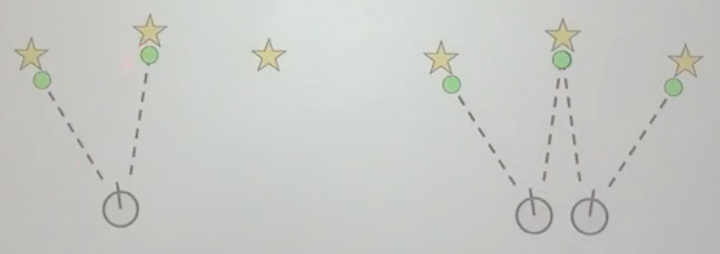
\includegraphics[scale=0.5]{ukcorresp}
\end{center}

Most approaches assume to have perfect data associations. This is unrealistic, but in fairness it is quite hard to track all possible data associations. A compromise would be to take into account a defined number of possible alternate estimations at each point.

\textbf{Static vs. dynamic environment}

There are approaches which explicitly allow the modelling of a dynamic environment, instead of taking the static assumption.

\textbf{Small vs. large uncertainty}

This is related to how much uncertainty the algorithm is willing and able to take into account at each stage and location.

\textbf{Active vs. passive SLAM}

Passive SLAM assumes that there is an external data stream being input, and simply follows it. In active SLAM, the robot can be thought of as exploring the environment on its own.

\textbf{Any-time and any-space SLAM}

This gives a pre-defined limit to the memory and time allowed for the robot to make its estimations at each stage.

\textbf{Single-robot vs. multi-robot SLAM}

With more robots, data associations can be sent from one robot to another, increasing accuracy.

\subsection{Motion and observation models}

The motion model works to estimate the probability of a certain $x_t$ given all data collected up to the point $t$. The observation model estimates the likelihood of a certain observation being correct, given knowledge of the robot's pose and currently known landmarks.

\textbf{Motion model}

\begin{center}
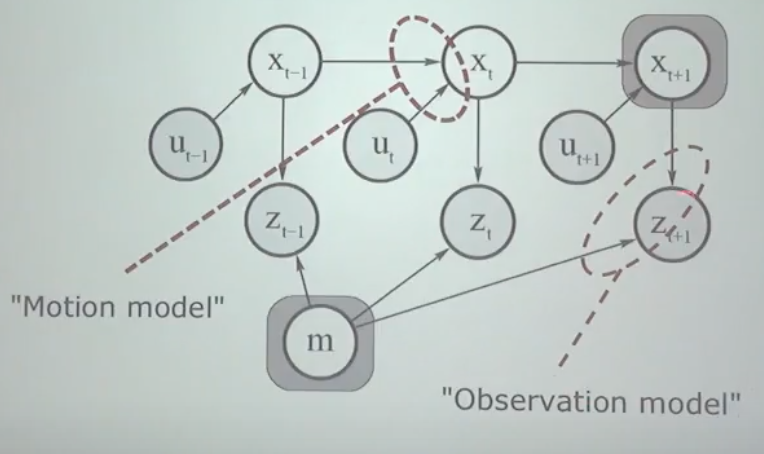
\includegraphics[scale=0.5]{motandobs}
\end{center}

\begin{center}
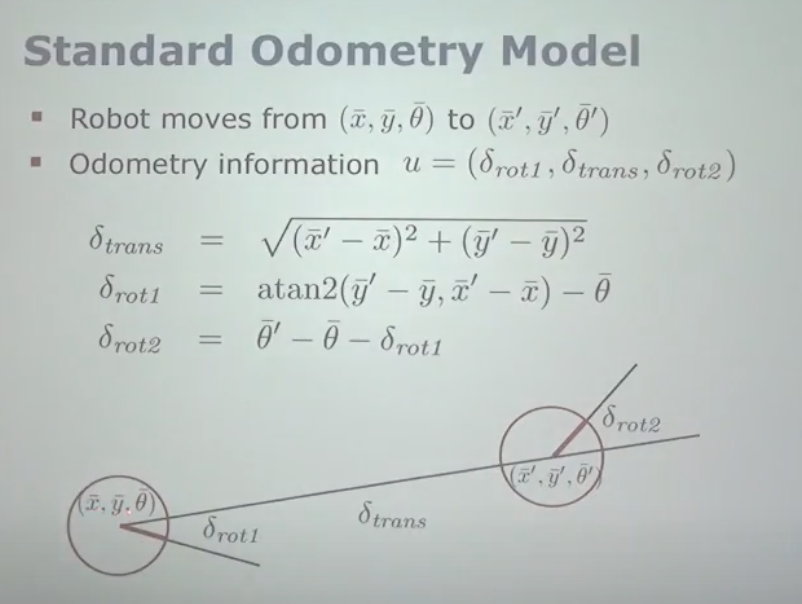
\includegraphics[scale=0.6]{stdod}
\end{center}

Here, the motion model effects the transformation from the first pose to second is by a first rotation, a translation, and then a second rotation.

\textbf{Observation model}

This refers to what one expects the world map to look like, given current estimations. It includes both Gaussian and non-Gaussian models.

\pagebreak

%%%%%%%%%%%%%%%%%%%%%%%%%%%%%%%%%%%%%%%%%%%%%

\section{Homogeneous coordinates}

\subsection{Motivation}

\begin{itemize}
    \item Cameras generate a projected image of the world
    \item Euclidean geometry is quite sub-optimal when it comes to describing the central projection
    \item Projective geometry is an alternative algebraic representation of geometric objects and transformations
\end{itemize}

Sensors may sometimes not measure the distance to obstacles, but instead just the orientation of the obstacle with respect to the heading of the robot. For example, cameras know which pixels correspond to which angular orientation, and thus generate a projection of the 3D world onto a 2D image, without knowing exactly how far each point is.

Such an approach is quite hard to implement via Euclidean geometry due to complexities in obtaining the correct coordinates. Hence to make the math simpler, projective geometry is used (it does not change the relations between the objects and the surrounding space).

\subsection{Homogeneous coordinates}

\begin{itemize}
    \item Points at infinity can be represented using finite coordinates - which is much harder to do in Euclidean geometry
    \item A single matrix can be used to represent affine as well as projective transformations
\end{itemize}

Affine transformations include rotations, translations, shearing and scale changes - being able to implement all of these in the same way, using a single matrix, is quite convenient. This is one of the main reasons for using homogeneous coordinates (HC).

\textbf{Definition}

The representation $X$ of a geometric object is homogeneous if $X$ and $\lambda X$ represent the same object for $\lambda \neq 0$.

\begin{equation*}
X =
\begin{bmatrix}
u\\v\\w
\end{bmatrix}
=
\begin{bmatrix}
wx\\wy\\w
\end{bmatrix}
=
\begin{bmatrix}
x\\y\\1
\end{bmatrix}
\end{equation*}

That is, we have some vector $X$, and this vector, as well as any scalar multiple of it, should refer to the same object.

\textbf{Homogeneous to Euclidean}

\begin{equation*}
X =
\begin{bmatrix}
u\\v\\w
\end{bmatrix}
=
\begin{bmatrix}
wx\\wy\\w
\end{bmatrix}
=
\begin{bmatrix}
x\\y\\1
\end{bmatrix}
,   X =
\begin{bmatrix}
x\\y
\end{bmatrix}
\end{equation*}

\begin{equation*}
\begin{bmatrix}
u\\v\\w
\end{bmatrix}
=
\begin{bmatrix}
u/w\\v/w\\1
\end{bmatrix}
\longrightarrow
\begin{bmatrix}
u/w\\v/w
\end{bmatrix}
=
\begin{bmatrix}
x\\y
\end{bmatrix}
\end{equation*}

Essentially, to map from the Euclidean space to HC, one simply adds a new dimension to the Euclidean 2D vector, which takes the value 1. For the reverse process, we normalize the first two dimensions using the third dimension.

\begin{center}
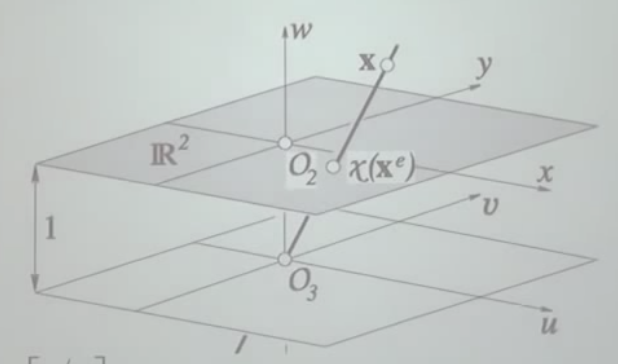
\includegraphics[scale=0.7]{hced}
\end{center}

Whichever Z-plane the HC point lies at on the line shown, it will ultimately intersect the base 2D plane at the same point. This is the principle of using HC - any point on that line can be used to represent the original required point.

\textbf{Centers of the coordinate system (for 2D and 3D)}

\begin{equation*}
O_2 =
\begin{bmatrix}
0\\0\\1
\end{bmatrix}
\: O_3 = 
\begin{bmatrix}
0\\0\\0\\1
\end{bmatrix}
\end{equation*}

\textbf{Infinitely distant objects}

Using HC, it is now possible to explicitly model infinitely distant points with finite coordinates:

\begin{equation*}
X_{\infty} =
\begin{bmatrix}
u \\ v \\ 0
\end{bmatrix}
\end{equation*}

Being able to do this is an extremely useful tool when working with bearing-only sensors such as cameras which don't measure distances as such. Such a model also makes it much easier to check if lines are parallel or orthogonal, without having to go into the rigours of their representations.

\textbf{3D points}

This concept of transformation is analogous for 3D points as well, making use of a fourth dimension here.

\begin{equation*}
X = 
\begin{bmatrix}
u\\v\\w\\t
\end{bmatrix}
=
\begin{bmatrix}
u/t\\v/t\\w/t\\1
\end{bmatrix}
\longrightarrow
\begin{bmatrix}
u/t\\v/t\\w/t
\end{bmatrix}
\end{equation*}

\subsection{Transformations}

One can now represent all required transformations using matrices. The only condition is that the matrix used should be invertible, which will be taken care of if the matrices are designed in the ways shown in this section.

A projective transformation is an invertible linear mapping. As already discussed, the $\lambda$ used in the various matrices used to effect the transformations which will be shown, can take any value. 

Matrices can thus be used to represent the various types of affine transformations mentioned earlier in a simple and efficient manner. Thus using HC to effect these is hugely beneficial, rather than having to add and multiply together separate vectors in a messy manner as is done with Euclidean coordinates.

\textbf{Translation}

\begin{center}
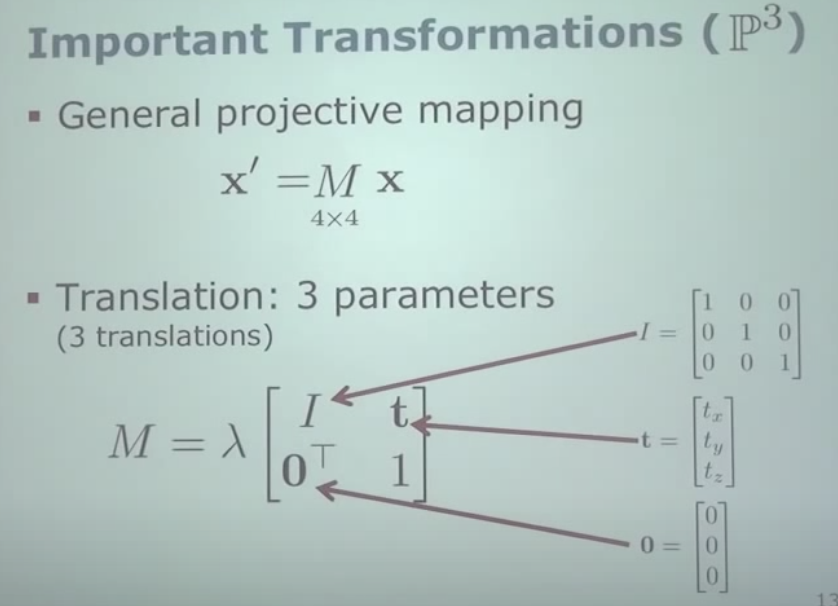
\includegraphics[scale=0.5]{3dtran}
\end{center}

Here the vector $\mathbf{t}$ represents the required translation.

\textbf{Rotation}

\begin{equation*}
M = \lambda
\begin{bmatrix}
R && 0 \\ 0^T && 1
\end{bmatrix}
\end{equation*}

The rotation matrix is the usual one used to rotate around an axis in Euclidean coordinates - it has three parameters for the 3D coordinate system due to the presence of three rotation axes.

\begin{center}
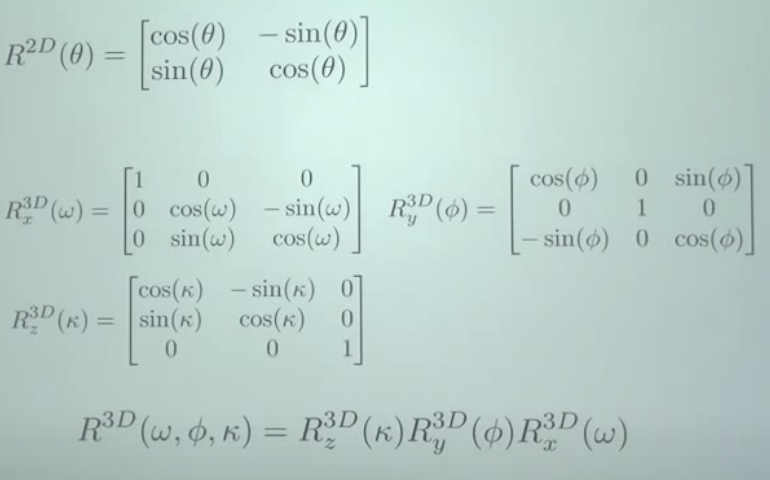
\includegraphics[scale=0.5]{rotmats}
\end{center}

The $\kappa$ matrix effects the rotation around the $X$ axis. Similarly, the $\phi$ matrix is for the $Y$ axis, and the $\omega$ matrix is for the $Z$ axis. Multiplying these together as shown effects all three rotations simultaneously.

\textbf{Rigid body transformation}

Such a transformation has 6 parameters: 3 for rotation and 3 for translation. This is the main type of transformation which is used in robot mapping.

\begin{equation*}
M = \lambda
\begin{bmatrix}
R && t \\
0^T && 1
\end{bmatrix}
\end{equation*}

where $R$ and $t$ represent the rotation matrix and translation vector respectively.

\textbf{Other important transformations}

\begin{center}
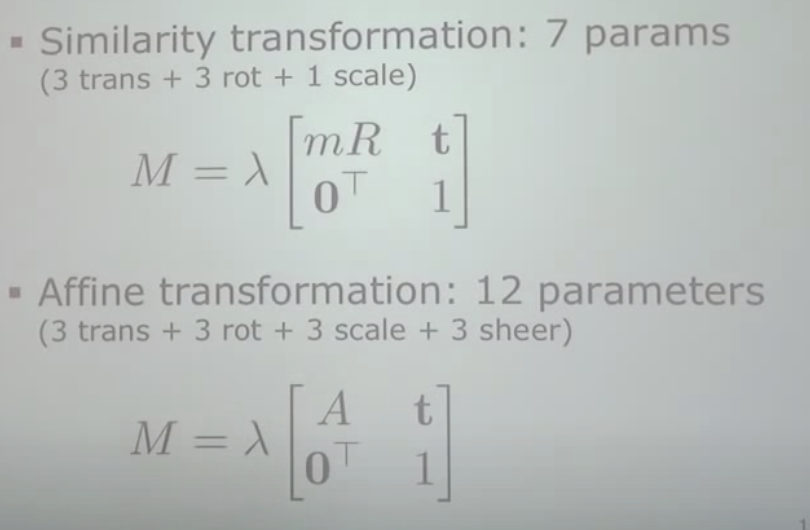
\includegraphics[scale=0.5]{imptras1}
\end{center}

The parameter $m$ in the first equation above is used to scale the object being transformed. It cannot be pre-multiplied with the entire matrix, otherwise it would be scaled away by the $\lambda$.

\textbf{Inverting a transformation}

\begin{equation*}
    X' = MX
\end{equation*}
\begin{equation*}
    X' = M^{-1}X
\end{equation*}

Note: $M$ is always invertible, given it is constructed according to the methods that have been shown.

\textbf{Chaining transformations}

The matrix product is not commutative, so one must be careful in which order the transformations are chained.

\begin{equation*}
    X' = M_1M_2X \neq M_2M_1X
\end{equation*}

\pagebreak

%%%%%%%%%%%%%%%%%%%%%%%%%%%%%%%%%%%%%%%%%%%%%%%%%

\section {The Bayes Filter}

\subsection{State estimation}

The Bayes filter is a method of doing state estimation. One has observation data ($z$), as well as control data - the set of commands sent to the robot ($u$). Using these, we want to estimate the state of the world - the pose of the robot, the location of landmarks, etc.

\begin{equation*}
    Goal: p(x| z,u)
\end{equation*}

If we have no data yet, we begin with a uniform distribution - every state is equally likely. As one acquires more data and executes actions, one gets more certain about the state. Ultimately the aim is to obtain a peak-type distribution of the state.

The probability here is estimated using Bayes rule. One observation and one control are integrated at a time, recursively, to obtain the state of the system.

\subsection{Recursive Bayes Filter }

\begin{equation*}
    bel(x_t) = p(x_t | z_{1:t}, u_{1:t})
\end{equation*}

Here, `bel' or `belief', refers to the estimation of the probability distribution of $x_t$, given a sequence of sensor commands and a sequence of observations made up to that point in time $t$. Applying Bayes rule to this distribution, we get

\begin{equation*}
    bel(x_t) = \eta * p(z_t | x_t, z_{1:t-1}, u_{1:t})* p(x_t | z_{1:t-1}, u_{1:t})
\end{equation*}

where $\eta$ is a normalizing term.

In this new definition of $bel$, Bayes rule has been simply applied  to make $z_t$ the dependent variable in the probability estimation. Now, one applies the Markov assumption in order to simplify the first term.

\textbf{The Markov assumption}: given you know the current state of the world, you can estimate the probability distribution of the current distribution without considering any previous controls executed or observations made.

Applying this assumption to our definition of $bel$, we now get

\begin{equation*}
    bel(x_t) = \eta * p(z_t | x_t) * p(x_t | z_{1:t-1}, u_{1:t})
\end{equation*}

Now, looking at the second term of $bel$, it estimates the current state of the system, given observations up to time $t-1$, plus all the commands executed up to that point. Thus it is like having a complete state estimate up to $t-1$, plus executing a motion command.

Using the law of total probability, we introduce the variable $x_{t-1}$ to represent the state of the system at the time $t-1$, the just previous time step. The second term will thus turn into an integral.

\begin{equation*}
    bel(x_t) = \eta * p(z_t | x_t)  \int_{x_{t-1}} p(x_t | x_{t-1}, z_{1:t-1}, u_{1:t}) * p(x_{t-1} | z_{1:t-1}, u_{1:t}) dx_{t-1}
\end{equation*}

This transformation has been effected based on the rule of total probability, which makes use of a continuous known second probability distribution to estimate the first required one as follows:

\begin{equation*}
    P(A) = \int_B P(A|B) * P(B) dB
\end{equation*}

Now the Markov assumption is once again applied, this time to the first term of the integral - if one wants to know the current state of the world, and given that one knows the previous time step state, everything seen or done before that time step can be ignored.

So all the observations can be gotten rid of, and all the commands can be gotten rid of too, \textit{except} $u_t$, as we need the current command to update the state from $x_{t-1}$ to $x_t$. The equation now changes to

\begin{equation*}
    bel(x_t) = \eta * p(z_t | x_t)  \int_{x_{t-1}} p(x_t | x_{t-1}, u_t) * p(x_{t-1} | z_{1:t-1}, u_{1:t}) dx_{t-1}
\end{equation*}

So essentially, the new first term of the integral indicates that given one knows the previous time step's state, and the current command is executed, a probability distribution for the current state can be obtained.

Next, turning to the second term of the integral, one can assume that one does not need $u_t$ to estimate $x_{t-1}$, as $u_t$ will be executed in the future, not at the current time.

However, this is not always the case - knowing what command the robot will execute in the future can in certain circumstances allow one to make a better prediction of the current state. 

For example, if one has to make an estimate between a pose which has an obstacle $50 cm$ in front, and a pose which has its path clear, and one knows that the next command is to move $ 1 m$ ahead, then the current pose is more likely to be closer to the latter option of the estimate. 

Yet, this possibility is ignored - the assumption is made that the command executed in the future has no relevance to the current state of the system.

\begin{equation*}
    bel(x_t) = \eta * p(z_t | x_t)  \int_{x_{t-1}} p(x_t | x_{t-1}, u_t) * p(x_{t-1} | z_{1:t-1}, u_{1:t-1}) dx_{t-1}
\end{equation*}

Now, looking again at the second term of the integral, and looking back to the very first definition of $bel$ (i.e.  $bel(x_t) = p(x_t | z_{1:t}, u_{1:t})$  the second term is clearly of the same form as the definition, only defined for $t-1$ instead of $t$. And thus we obtain the recursive term in this definition.

\begin{equation*}
    bel(x_t) = \eta * p(z_t | x_t)  \int_{x_{t-1}} p(x_t | x_{t-1}, u_t) * bel(x_{t-1}) dx_{t-1}
\end{equation*}

So one now has a recursive update scheme which allows one to estimate the current state of the system based on the previous state $x_{t-1}$, the current motion command executed $u_t$, and the current observation obtained $z_t$.

This is the spirit of online SLAM - not needing any command or observation made in the future (taking into account the assumptions made).

\subsection{Prediction and correction}

The Bayes filter can be written as a two step process.

\textbf{Prediction step}

\begin{equation*}
    \overline{bel}(x_t) = \int_{x_{t-1}} p(x_t | x_{t-1}, u_t) * bel(x_{t-1}) dx_{t-1}
\end{equation*}

The prediction step takes into account the command executed. It entails integration over all the possible states in the estimation made for $x_{t-1}$.

\textbf{Correction step}

\begin{equation*}
    bel(x_t) = \eta * p(z_t | x_t) * \overline{bel}(x_t)
\end{equation*}

The correction step takes into account the observation made, and increases the likelihood of those states found in the prediction step which agree more with the sensors' observations. The normalizing term ensures that the sum or integral of all possible states equals to 1.

The prediction and correction steps also connect to the motion and observation models as such.

\begin{center}
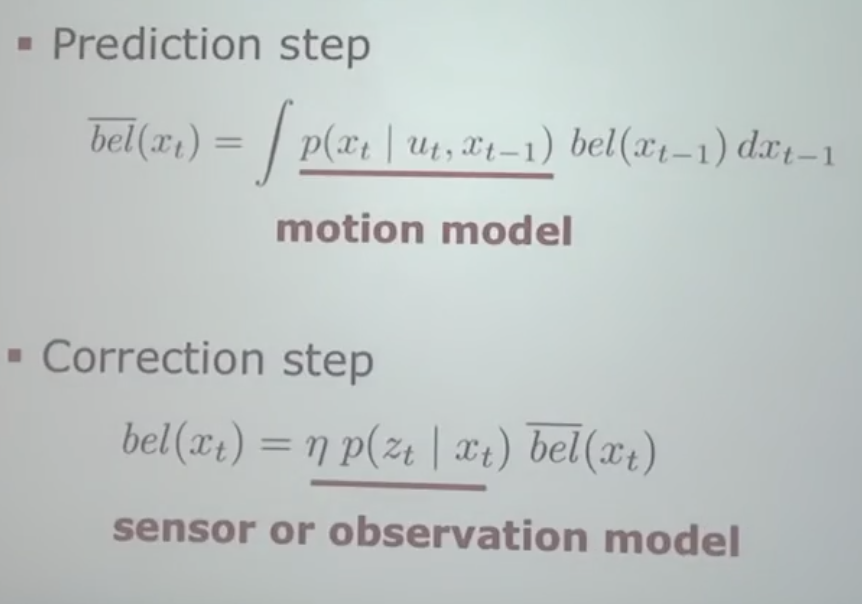
\includegraphics[scale=0.5]{pcmodels}
\end{center}

\subsection{Different realizations}

The Bayes filter is a framework for recursive state estimation, but it doesn't specify exactly how we should go about calculating the defined integrals, or which assumptions to take into account while doing so.

Properties that influence the way the filter is implemented include:
\begin{itemize}
    \item Linear vs. non-linear models for motion and observation
    \item Type of distribution: e.g. Gaussian vs. uniform
    \item Parametric vs. non-parametric filters
\end{itemize}

Hence, there are several variants of the Bayes filter. Two important ones which will be discussed here are the Kalman filter and the Particle filter.

\textbf{Kalman filter}
\begin{itemize}
    \item Gaussian
    \item Linear or linearized models
\end{itemize}

\textbf{Particle filter}
\begin{itemize}
    \item Non-parametric
    \item Arbitrary models (sampling required)
\end{itemize}

The Kalman filter is highly optimised for systems that meet its specific requirements, and gives quite precise estimations. However, a robot's motion is often non-linear, and so in order to be able to take into account a wider range of states and state changes, the Particle filter is frequently used, though it has an increased computational cost.

\subsection{Motion model}

\begin{equation*}
    \overline{bel}(x_t) = \int_{x_{t-1}} \underline{p(x_t | x_{t-1}, u_t)} * bel(x_{t-1}) dx_{t-1}
\end{equation*}

To recap, this model looks into how to estimate the current state of the system, given the previous state and the command that was just executed.

Robot motion is inherently uncertain. The requirement is to be able to model the motion, given the uncertainty, since even small errors in the odometry information become big when accumulated over time.

\textbf{Probabilistic motion models}

Such models specify a posterior probability that action $u_t$ carries the robot from $x_{t-1}$ to $x_t$:

\begin{equation*}
    p(x_t | u_t, x_{t-1})
\end{equation*}

There are two different kind of models which can implement such a distribution.

\begin{enumerate}

    \item \textbf{Odometry-based model}: encoders are attached to the wheels of the robot, and they count the revolutions of the wheels. This gives one an estimate of where the robot is going. However, it can be inaccurate when the wheel dimensions don't match or the ground is uneven, causing drift. This is the easier-to-handle model of the two.
    
    \begin{center}
    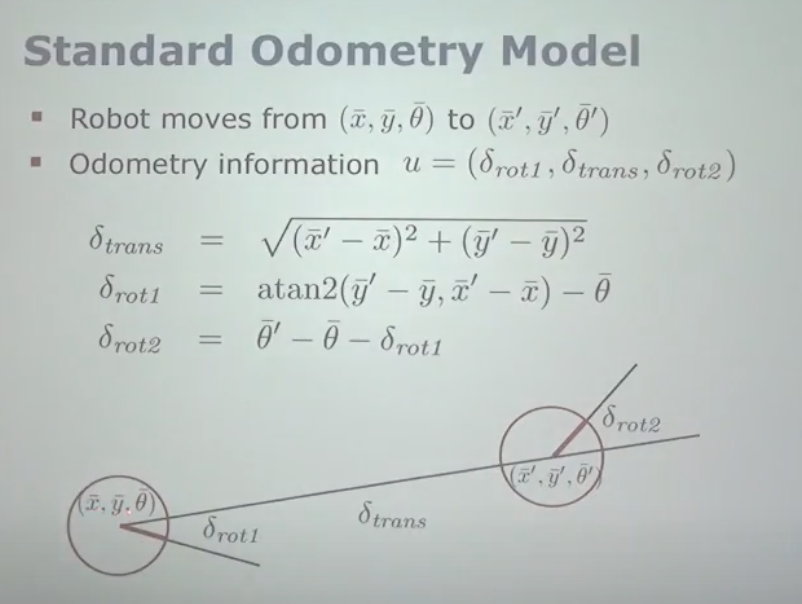
\includegraphics[scale=0.5]{stdod}
    \end{center}
    
    Suppose one is introducing Gaussian errors to the individual three components (rotation, translation, rotation) in the system.
    
    \begin{center}
    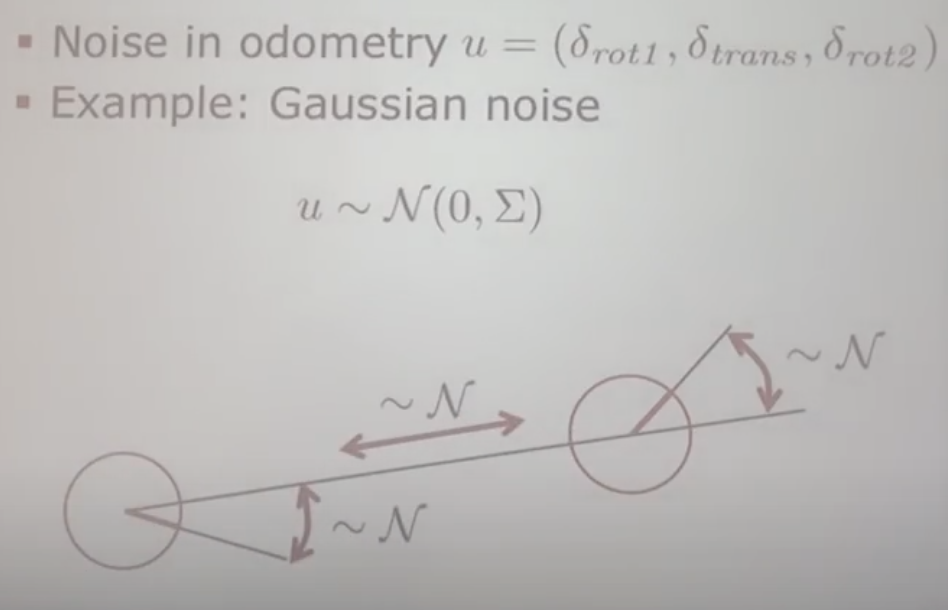
\includegraphics[scale=0.5]{odgaus}
    \end{center}
    
    However, the net error produced does not have a Gaussian distribution, due to the non-linear relations between each step. This leads to the production of banana-shaped distributions, which are better represented as histograms. This is the standard model which is used in most cases.
    
    \item \textbf{Velocity-based model}: encoders are not available. Velocity commands are instead sent to the system, and it is assumed that the system follows these commands to a certain accuracy. Used more in systems such as flying vehicles, or humanoid bots with legs.
    
    This model assumes that the motion command sent to the robot consists of two velocities - translational and rotational. The ideal result is the robot driving along a circular arc for short time intervals, as shown.
    
    \begin{center}
    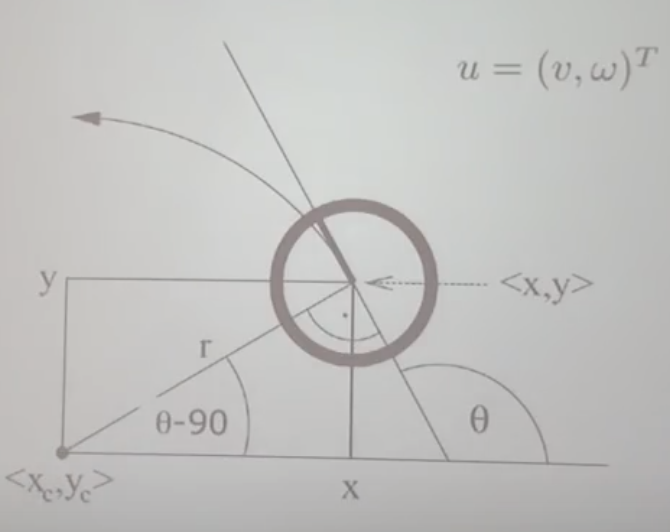
\includegraphics[scale=0.5]{velmodel}
    \end{center}
    
    The model assumes that there only a discrete number of opportunities to change the velocities, due to the discrete time steps at which the commands are sent to the robot. However, this is not always the case - there will be delays in executing the commands, so the time intervals will not always match - yet this is the assumption that is followed.
    
    \begin{itemize}
        \item Robot moves from $(x, y, \theta)$ to $(x', y', \theta ')$
        \item Velocity information $u = (v, w)$
    \end{itemize}
    
    \begin{equation*}
        \begin{pmatrix}
        x' \\ y' \\ \theta '
        \end{pmatrix}
        =
        \begin{pmatrix}
        x \\ y \\ \theta
        \end{pmatrix}
        +
        \begin{pmatrix}
        - \frac{v}{w} sin\theta + \frac{v}{w} sin (\theta + \omega \Delta t)
        \\ \frac{v}{w} cos\theta - \frac{v}{w} cos (\theta + \omega \Delta t) 
        \\ \omega \Delta t
        \end{pmatrix}
    \end{equation*}
    
    where $\theta + \omega \Delta t$ is the current orientation of the robot.
    
    Comparing the velocity-based model to the odometry-based model, the former has a translational and a rotational velocity, whereas the latter has a rotation, translation, and then another rotation. So essentially the difference is two parameters vs. three parameters. 

    Thus, in the velocity-based model, the circle constrains the final orientation. So one needs an additional term to account for this orientation. The fix is to introduce an additional noise term on the final orientation.
    
    \begin{equation*}
            \begin{pmatrix}
            x' \\ y' \\ \theta '
            \end{pmatrix}
            =
            \begin{pmatrix}
            x \\ y \\ \theta
            \end{pmatrix}
            +
            \begin{pmatrix}
            - \frac{v}{w} sin\theta + \frac{v}{w} sin (\theta + \omega \Delta t)
            \\ \frac{v}{w} cos\theta - \frac{v}{w} cos (\theta + \omega \Delta t) 
            \\ \omega \Delta t + \gamma \Delta t
            \end{pmatrix}
    \end{equation*}
    
    The $\gamma$ term introduced thus indicates how much rotation is required in the end to achieve the final orientation.
    
    The probability distributions produced by the velocity-based model are similar to the odometry-based ones. The main difference is that the estimates of the velocity-based models are much more noisy, hence the odometry-based model gives more accurate estimates.
    
\end{enumerate}

\subsection{Sensor model}

\begin{equation*}
    bel(x_t) = \eta * \underline{p(z_t | x_t)} * \overline{bel}(x_t)
\end{equation*}

This model obviously depends on which sensor being used. For example, the laser rangefinder, which gives the distance to the closest obstacle in a certain direction, is vastly different in the implementation of its model from a camera or a radar. The sensor first discussed here is the laser rangefinder (LR).

The LR typically has a mirror which rotates and reflects a laser beam, and a time of flight sensor which measures the time taken for the beam to bounce back from any obstacle to the receiver. So one obtains proximity measurements for various angular intervals at short time intervals.

\textbf{Model for laser scanners}

\begin{itemize}
    \item Scan $z$ consists of $K$ measurements.
    \begin{equation*}
        z_t = {z_t^1, \ldots , z_t^k}
    \end{equation*}
    \item Individual measurements are independent, given the robot position.
    \begin{equation*}
        p(z_t | x_t, m) = \prod_{i=1}^k p(z_t^i | x_t, m)
    \end{equation*}
\end{itemize}

Each observation consists of k proximity measurements. By knowing the orientation of the mirror, one can deduce the positions of the obstacles detected. 

Additionally, the measurements in each direction are assumed to be independent of each other. The probability distribution over the whole scan is taken to be the product of the distributions of the individual beams, which are modeled in each direction given that the robot knows its current state and what the environment looks like.

There are different ways for describing the individual beam distributions, which are so-called beam-based models. The simplest of these is the beam-endpoint model.

\textbf{Beam-endpoint model}

Suppose the robot sends out a beam in a particular direction. Depending on where the endpoint of the beam is calculated to be located, ignoring the data that the map provides in that specific direction, the position of the nearest obstacle in that direction is newly estimated.

From a physics point of view, this model may not seem quite sound. However, it works surprisingly well in practice. It is also extremely efficient to compute. This is because if one has their map, then this model simply creates a kind of Gaussian distribution indicating the position of each obstacle. It essentially boils down to looking up a value in an array - the further away one is from the obstacle, the lower the probability value retrieved, and vice versa.

The typical maps created by this are occupancy grid maps, which can also be converted to likelihood fields, where the brighter the map is at a point, the greater the probability of an obstacle being present at that location.

\textbf{Ray-cast model}

This is more expensive to compute, but physically more accurate. Suppose the map indicates that an obstacle is present at a certain location. The question the model asks is, what is the likelihood that one would measure a certain length, given it is known that the obstacle is four metres away?

The resulting distribution is a kind of mixture of four distributions:

\begin{center}
    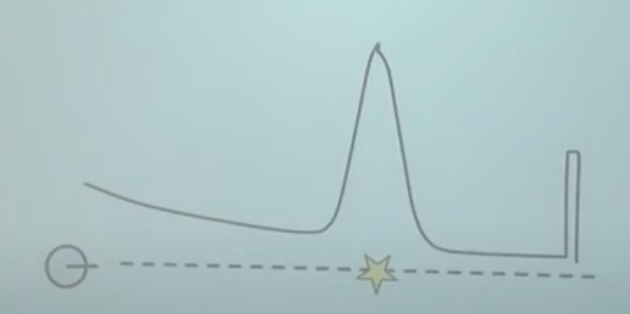
\includegraphics[scale=0.5]{raycast}
\end{center}

\begin{itemize}
    \item A gaussian distribution around the position of the actual obstacle
    \item A component which describes exponential decay - this allows one to account for dynamic obstacles, which only affect the primary obstacle's location up to the point where the obstacle itself is located
    \item A peak at the back, which is due to the maximum range reading of the sensor - the maximum distance the sensor can detect obstacles till
    \item A uniform distribution which accounts for any random remaining obstacles (will be covered in more detail later).
\end{itemize}

Thus, this model results in a distribution that is a lot more physically plausible than the one produced by the beam-endpoint model.

\textbf{Model for perceiving landmarks with range-bearing sensors}

\begin{itemize}
    \item Range bearing: $z_t^i = (r_t^i, \phi _t^i)^T$
    \item Robot's pose: $(x,y,\theta)^T$
    \item Observation of feature $j$ at location $(m_{j,x}, m_{j,y})^T$
\end{itemize}

\begin{equation*}
    \begin{pmatrix}
        r_t^i \\ \phi_t^i
    \end{pmatrix}
    =
    \begin{pmatrix}
        \sqrt{(m_{j,x} - x)^2 + (m_{j,y} - y)^2}
        \\ atan2(m_{j,y} - y, m_{j,x} - x) - \theta
    \end{pmatrix}
    + Q_t
\end{equation*}

The final model aims to give positions of distinct, defined landmarks using distance and orientation parameters. In these equations,

\begin{itemize}
    \item $r$ is the distance of the landmark measured by the LR
    \item $\phi$ is the orientation of the landmark with respect to the heading of the robot
    \item $(x,y,\theta)^T$ gives the current position of the robot
    \item $m_{j,x}, m_{j,y}$ give the location of the landmark in $x,y$ according to the current map $m$
    \item $Q_t$ refers to some noise; may be Gaussian or not
\end{itemize}

So for dense maps, the beam-endpoint and ray cast models will work better, and if one is working with defined landmarks, the perceiving model will be more suitable.

Altogether, given one is working with a particular odometry model, and has reached a certain position following the execution of a command, using any of these models allows an observation probability distribution to be estimated, and thus the Bayes filter to be applied.

\pagebreak

%%%%%%%%%%%%%%%%%%%%%%%%%%%%%%%%%%%%%%%%%

\end{document}